% Options for packages loaded elsewhere
\PassOptionsToPackage{unicode}{hyperref}
\PassOptionsToPackage{hyphens}{url}
%
\documentclass[
]{book}
\usepackage{amsmath,amssymb}
\usepackage{lmodern}
\usepackage{iftex}
\ifPDFTeX
  \usepackage[T1]{fontenc}
  \usepackage[utf8]{inputenc}
  \usepackage{textcomp} % provide euro and other symbols
\else % if luatex or xetex
  \usepackage{unicode-math}
  \defaultfontfeatures{Scale=MatchLowercase}
  \defaultfontfeatures[\rmfamily]{Ligatures=TeX,Scale=1}
\fi
% Use upquote if available, for straight quotes in verbatim environments
\IfFileExists{upquote.sty}{\usepackage{upquote}}{}
\IfFileExists{microtype.sty}{% use microtype if available
  \usepackage[]{microtype}
  \UseMicrotypeSet[protrusion]{basicmath} % disable protrusion for tt fonts
}{}
\makeatletter
\@ifundefined{KOMAClassName}{% if non-KOMA class
  \IfFileExists{parskip.sty}{%
    \usepackage{parskip}
  }{% else
    \setlength{\parindent}{0pt}
    \setlength{\parskip}{6pt plus 2pt minus 1pt}}
}{% if KOMA class
  \KOMAoptions{parskip=half}}
\makeatother
\usepackage{xcolor}
\IfFileExists{xurl.sty}{\usepackage{xurl}}{} % add URL line breaks if available
\IfFileExists{bookmark.sty}{\usepackage{bookmark}}{\usepackage{hyperref}}
\hypersetup{
  pdftitle={VICAL Guide: VEGETATION INDICES CALCULATOR},
  pdfauthor={INIFAP: Sergio Jiménez-Jiménez; Mariana Marcial-Pablo; Waldo Ojeda-Bustamante; Ernesto Sifuentes-Ibarra; Marco Inzunza-Ibarra, Ignacio Sánchez-Cohen},
  pdflang={en},
  hidelinks,
  pdfcreator={LaTeX via pandoc}}
\urlstyle{same} % disable monospaced font for URLs
\usepackage[margin=2cm]{geometry}
\usepackage{color}
\usepackage{fancyvrb}
\newcommand{\VerbBar}{|}
\newcommand{\VERB}{\Verb[commandchars=\\\{\}]}
\DefineVerbatimEnvironment{Highlighting}{Verbatim}{commandchars=\\\{\}}
% Add ',fontsize=\small' for more characters per line
\usepackage{framed}
\definecolor{shadecolor}{RGB}{248,248,248}
\newenvironment{Shaded}{\begin{snugshade}}{\end{snugshade}}
\newcommand{\AlertTok}[1]{\textcolor[rgb]{0.94,0.16,0.16}{#1}}
\newcommand{\AnnotationTok}[1]{\textcolor[rgb]{0.56,0.35,0.01}{\textbf{\textit{#1}}}}
\newcommand{\AttributeTok}[1]{\textcolor[rgb]{0.77,0.63,0.00}{#1}}
\newcommand{\BaseNTok}[1]{\textcolor[rgb]{0.00,0.00,0.81}{#1}}
\newcommand{\BuiltInTok}[1]{#1}
\newcommand{\CharTok}[1]{\textcolor[rgb]{0.31,0.60,0.02}{#1}}
\newcommand{\CommentTok}[1]{\textcolor[rgb]{0.56,0.35,0.01}{\textit{#1}}}
\newcommand{\CommentVarTok}[1]{\textcolor[rgb]{0.56,0.35,0.01}{\textbf{\textit{#1}}}}
\newcommand{\ConstantTok}[1]{\textcolor[rgb]{0.00,0.00,0.00}{#1}}
\newcommand{\ControlFlowTok}[1]{\textcolor[rgb]{0.13,0.29,0.53}{\textbf{#1}}}
\newcommand{\DataTypeTok}[1]{\textcolor[rgb]{0.13,0.29,0.53}{#1}}
\newcommand{\DecValTok}[1]{\textcolor[rgb]{0.00,0.00,0.81}{#1}}
\newcommand{\DocumentationTok}[1]{\textcolor[rgb]{0.56,0.35,0.01}{\textbf{\textit{#1}}}}
\newcommand{\ErrorTok}[1]{\textcolor[rgb]{0.64,0.00,0.00}{\textbf{#1}}}
\newcommand{\ExtensionTok}[1]{#1}
\newcommand{\FloatTok}[1]{\textcolor[rgb]{0.00,0.00,0.81}{#1}}
\newcommand{\FunctionTok}[1]{\textcolor[rgb]{0.00,0.00,0.00}{#1}}
\newcommand{\ImportTok}[1]{#1}
\newcommand{\InformationTok}[1]{\textcolor[rgb]{0.56,0.35,0.01}{\textbf{\textit{#1}}}}
\newcommand{\KeywordTok}[1]{\textcolor[rgb]{0.13,0.29,0.53}{\textbf{#1}}}
\newcommand{\NormalTok}[1]{#1}
\newcommand{\OperatorTok}[1]{\textcolor[rgb]{0.81,0.36,0.00}{\textbf{#1}}}
\newcommand{\OtherTok}[1]{\textcolor[rgb]{0.56,0.35,0.01}{#1}}
\newcommand{\PreprocessorTok}[1]{\textcolor[rgb]{0.56,0.35,0.01}{\textit{#1}}}
\newcommand{\RegionMarkerTok}[1]{#1}
\newcommand{\SpecialCharTok}[1]{\textcolor[rgb]{0.00,0.00,0.00}{#1}}
\newcommand{\SpecialStringTok}[1]{\textcolor[rgb]{0.31,0.60,0.02}{#1}}
\newcommand{\StringTok}[1]{\textcolor[rgb]{0.31,0.60,0.02}{#1}}
\newcommand{\VariableTok}[1]{\textcolor[rgb]{0.00,0.00,0.00}{#1}}
\newcommand{\VerbatimStringTok}[1]{\textcolor[rgb]{0.31,0.60,0.02}{#1}}
\newcommand{\WarningTok}[1]{\textcolor[rgb]{0.56,0.35,0.01}{\textbf{\textit{#1}}}}
\usepackage{longtable,booktabs,array}
\usepackage{calc} % for calculating minipage widths
% Correct order of tables after \paragraph or \subparagraph
\usepackage{etoolbox}
\makeatletter
\patchcmd\longtable{\par}{\if@noskipsec\mbox{}\fi\par}{}{}
\makeatother
% Allow footnotes in longtable head/foot
\IfFileExists{footnotehyper.sty}{\usepackage{footnotehyper}}{\usepackage{footnote}}
\makesavenoteenv{longtable}
\usepackage{graphicx}
\makeatletter
\def\maxwidth{\ifdim\Gin@nat@width>\linewidth\linewidth\else\Gin@nat@width\fi}
\def\maxheight{\ifdim\Gin@nat@height>\textheight\textheight\else\Gin@nat@height\fi}
\makeatother
% Scale images if necessary, so that they will not overflow the page
% margins by default, and it is still possible to overwrite the defaults
% using explicit options in \includegraphics[width, height, ...]{}
\setkeys{Gin}{width=\maxwidth,height=\maxheight,keepaspectratio}
% Set default figure placement to htbp
\makeatletter
\def\fps@figure{htbp}
\makeatother
\setlength{\emergencystretch}{3em} % prevent overfull lines
\providecommand{\tightlist}{%
  \setlength{\itemsep}{0pt}\setlength{\parskip}{0pt}}
\setcounter{secnumdepth}{5}
\ifLuaTeX
\usepackage[bidi=basic]{babel}
\else
\usepackage[bidi=default]{babel}
\fi
\babelprovide[main,import]{english}
% get rid of language-specific shorthands (see #6817):
\let\LanguageShortHands\languageshorthands
\def\languageshorthands#1{}
\usepackage{booktabs}
\usepackage{amsthm}
\makeatletter
\def\thm@space@setup{%
  \thm@preskip=8pt plus 2pt minus 4pt
  \thm@postskip=\thm@preskip
}
\makeatother
\usepackage{titling}
\pretitle{\begin{center} 
\includegraphics[width=2in,height=2in]{./images/LOGO2.png}\LARGE\\}
\posttitle{\end{center}}
\ifLuaTeX
  \usepackage{selnolig}  % disable illegal ligatures
\fi
\usepackage[]{natbib}
\bibliographystyle{apalike}

\title{VICAL Guide: VEGETATION INDICES CALCULATOR}
\author{INIFAP: Sergio Jiménez-Jiménez; Mariana Marcial-Pablo; Waldo Ojeda-Bustamante; Ernesto Sifuentes-Ibarra; Marco Inzunza-Ibarra, Ignacio Sánchez-Cohen}
\date{2022-07-18}

\begin{document}
\maketitle

{
\setcounter{tocdepth}{1}
\tableofcontents
}
\hypertarget{welcome}{%
\chapter*{Welcome}\label{welcome}}
\addcontentsline{toc}{chapter}{Welcome}

This site is a guide to use the \textbf{VICAL} tool developed within Google Earth Engine (GEE). VICAL calculates \textbf{online} 23 vegetation indices (commonly used in agricultural applications) of any polygon(s) in the world (digitized by the user or vector file) using LandSat and Sentinel-2 images. This is done without the user downloading/uploading satellite images of writing a single line of code, they just need to have an internet connection.

A web application is also available \url{https://inifapcenidraspa.users.earthengine.app/view/vical}.

\begin{figure}

{\centering 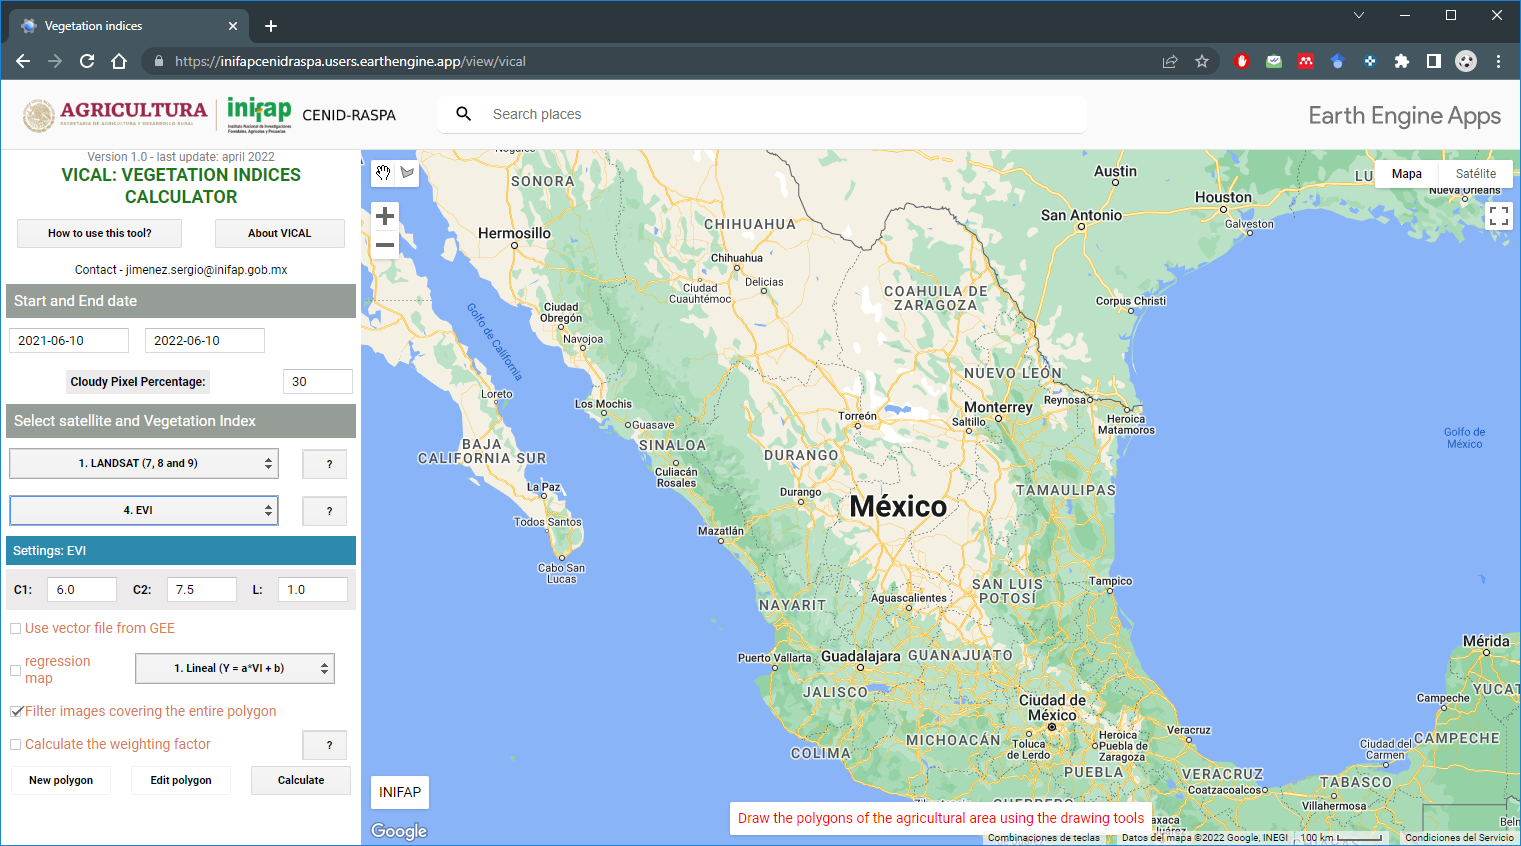
\includegraphics[width=0.9\linewidth]{./images/Captura2} 

}

\caption{Vista principal de VICAL}\label{fig:fig2}
\end{figure}

This work was developed by researchers from \textbf{INIFAP CENID-RASPA} and \textbf{CEVAF}. Among the improvements planned for VICAL is that are intended for VICAL is that through experimentation the calibration of biophysical variables of interest for various crops is achieved using \emph{vegetation indices (IV)}; and these results are available in \textbf{VICAL} to be useful to other people and thus they can easily monitor variables related to irrigation engineering.

\emph{Please check back occasionally for new GEE applications, example scripts, and VICAL updates. You might try doing a hard refresh on the site to make sure you see recent changes (what you're looking at might be a previously cached version of the site)}

\emph{If you have any questions or suggestions or wish to participate in the project, you can write to the email \textbf{\href{mailto:jimenez.sergio@inifap.gob.mx}{\nolinkurl{jimenez.sergio@inifap.gob.mx}}}}

\hypertarget{intro}{%
\chapter{Introduction}\label{intro}}

This guide is intended to introduce the basics of running VICA and how to implement the libraries in any GEE Script. It describes the VICAL conceptual framework, the vegetation indices (VIs) considered and the images collections used to calculate it, how to run it, what the outputs are, and how they are formatted.

VICAL was developed within the GEE platform \url{https://earthengine.google.com/} and was coded in JavaScript from the Earth Engine Code Editor \url{https://code.earthengine.google.com/}.

\hypertarget{scopes}{%
\section{Scopes}\label{scopes}}

The design principles for \textbf{VICAL} were that it should provide for any area (defined by the user) where there is a Landsat or Sentinel-2 image, the estimation of different VIs applied in agriculture. In addition, to graph the VI time series for that area in the date range established by the user. \textbf{All without the user writing a single line of code within the GEE platform or performing image pre-processing.}

The VICAL tool has three main functions::

\textbf{1.-} calculation of 23 VIs with images (cloud-free) from Landsat (4, 5, 7, 8 and 9) and Sentinel-2 data from any user-defined area.

\textbf{2.-} VI time series plot for each polygon drawn by the user with Landsat and Sentinel-2 or both satellites.

\textbf{3.-} Regression maps (linear, quadratic, potential or exponential function) or weighting factor using VIs values.

In this tool, you can configure some VI coefficients such as EVI, SAVI, among others.

We believe that the \textbf{VICAL} tool saves time and avoids the trivial repetitive procedure associated with ``manual'' VI calculations (image download, processing, etc.), which requires different types of software, which can lead to human error.

VICAL can be used to quickly extract VIs values for calibration in agricultural biophysical variables.

\hypertarget{Sat}{%
\chapter{Satellites - Image Collection}\label{Sat}}

VICAL used the atmospherically corrected land surface reflectance images from Landsat (missions 4, 5, 7, 8 and 9, with images from 1982 to present) and Sentinel-2. Table \ref{tab:Sat} shows the properties of these image collections in the GEE.

\begin{table}

\caption{\label{tab:Sat}Image collection of Landsat and Sentinel-2 within the Google Earth Engine (GEE)}
\centering
\begin{tabular}[t]{lll}
\toprule
Sensor & Dataset.availability & Collection.ID\\
\midrule
Landsat-4 TM & 22/08/1982 - 24/06/1993 & LANDSAT/LT04/C02/T1\_L2\\
Landsat-5 TM & 16/03/1993 – 05/05/2012 & LANDSAT/LT05/C02/T1\_L2\\
Landsat-7 ETM+ & 01/01/1999-present & LANDSAT/ LC08 /C02/T1\_L2\\
Landsat-8 OLI & 11/04/2013- present & LANDSAT/LE07/C02/T1\_L2\\
Landsat-9 OLI-2 & 31/10/2021- present & LANDSAT/LC09/C02/T1\_L2\\
\addlinespace
Sentinel-2 (MSI) & 28/03/2017-present & COPERNICUS/S2\_SR\_HARMONIZED\\
\bottomrule
\end{tabular}
\end{table}

The location of the different spectral bands of these sensors is shown in Figure \ref{fig:figS1}.

\begin{figure}

{\centering 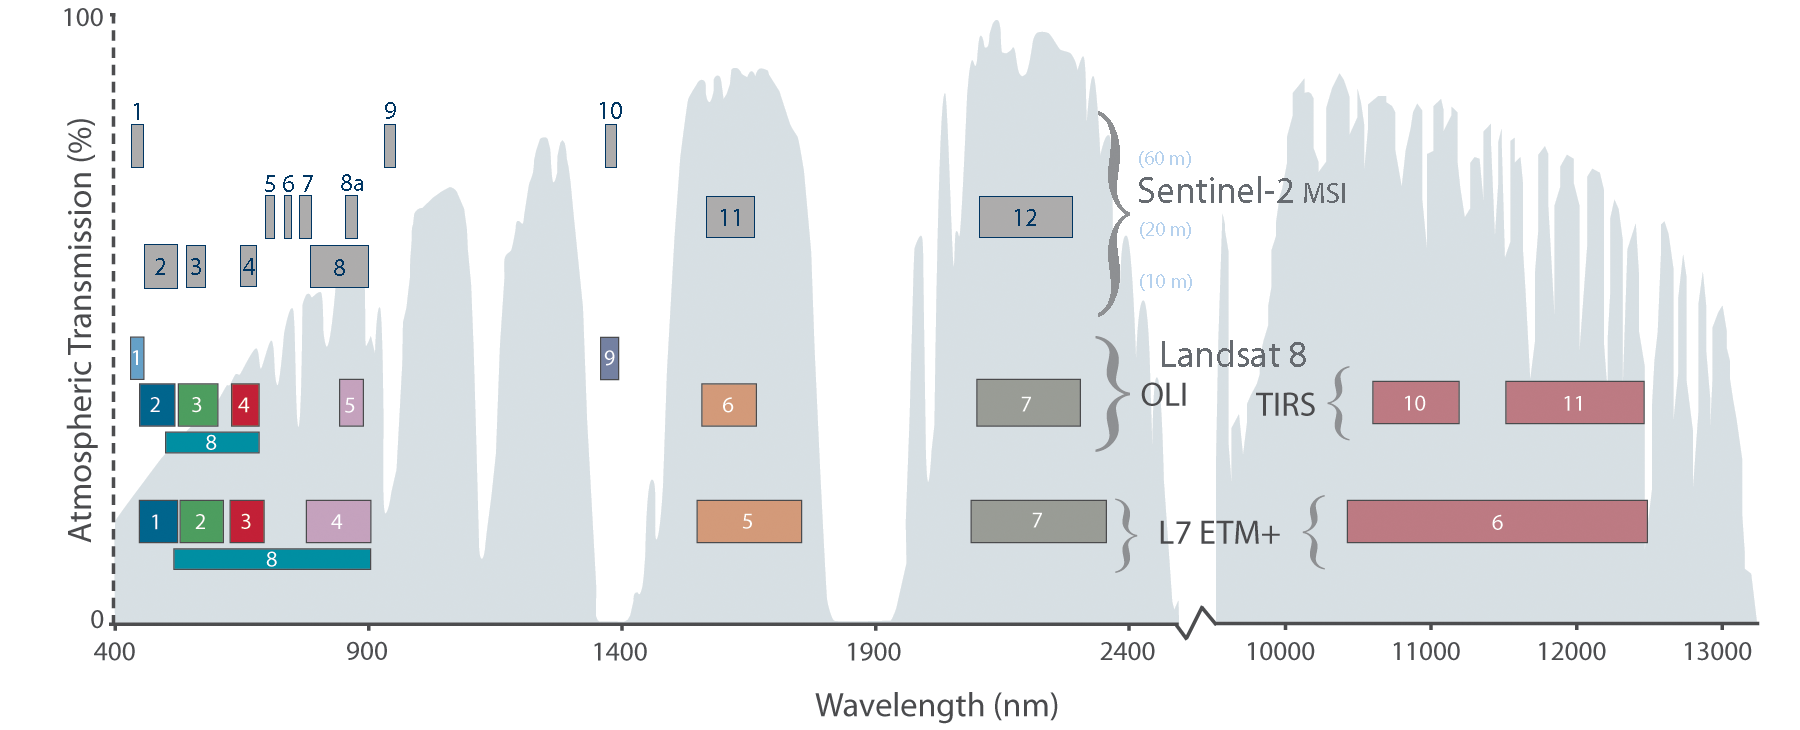
\includegraphics{./images/Figure21} 

}

\caption{Comparison of Landsat and Sentinel-2 and location of the spectral bands. The numbers indicate the number of spectral bands considered in each sensor [@NASA2021]}\label{fig:figS1}
\end{figure}

In VICAL, there are four calculation options in VICAL with these image collections: \textbf{(i) Landsat (7, 8 and 9), (ii) Sentinel-2, (iii) Landsat (7, 8 and 9) and Sentinel-2 and (iv) Landsat (4 and 5)}.

\hypertarget{Iveg}{%
\chapter{Vegetation Indices}\label{Iveg}}

The VIs allow the quantitative and functional relationship with different parameters or variables of the vegetation. There are 23 VIs considered in VICAL, these VIs are commonly used in agricultural applications \citep{Bannari2009},\citep{Xue2017}.

The names of these VIs, their mathematical expression as well as their abbreviation are shown in the following list:
\textbf{1: ARVI}: Atmospherically resistant vegetation index*
\[
ARVI = \frac{p(NIR-rb)}{NIR+rb};     
\]
\[
rb = {R-γ(B-R)}; \thinspace \thinspace  Default \thinspace value: \thinspace γ=1.0 
\]

\textbf{2: ATSAVI}: Adjusted transformed soil-adjusted vegetation index\emph{
\[
ATSAVI = \frac{a(NIR-aR-b)}{(R+aNIR-ab+X(1+a^2))};
\]
\[
\thinspace \thinspace  Default \thinspace value: \thinspace a= 1 ;\thinspace b=0; \thinspace X= 0.08      
\]
\textbf{3: DVI: } Difference vegetation index
\[
DVI = {(NIR-R)} ;   
\]
\textbf{4: EVI}}: Enhanced vegetation index
\[
EVI = \frac{2.5*(NIR-R)}{NIR+C_1 R-C_2 B+L};     
\]
\[
\thinspace \thinspace  Default \thinspace value: \thinspace C_1= 6.0 ;\thinspace C_2=7.5; \thinspace L= 1.0      
\]
\textbf{5: EVI2}*: Enhanced vegetation index
\[
EVI2 = \frac{2.5*(NIR-R)}{NIR+C_1 R+1}; \thinspace \thinspace  Default \thinspace value: \thinspace C_1= 2.4      
\]
\textbf{6: GNDVI}: Green normalized difference vegetation index
\[
GNDVI = \frac{NIR-G}{NIR+G};     
\]
\textbf{7: MSAVI2}: Modified soil adjusted vegetation index
\[
MSAVI2 = \frac{(2NIR+1)-\sqrt((2NIR+1)^2-8(NIR-R))}{2};     
\]
\textbf{8: MSI}: Moisture stress index
\[
MSI = \frac{SWIR_1}{NIR};     
\]
\textbf{9: MTVI}: Modified triangular vegetation index
\[
MTVI ={1.2[1.2*(NIR-G)-2.5*(R-G)]};     
\]

\textbf{10: MTVI2}: Modified triangular vegetation index-2
\[
MTVI2 = \frac{1.2[1.2*(NIR-G)-2.5*(R-G)]}{\sqrt((2NIR+1)^2-(6NIR-5\sqrt(R))-0.5)};     
\]
\textbf{11: NDTI}: Normalized difference tillage index (NDTI)
\[
NDTI = \frac{SWIR_1-SWIR_2}{SWIR_1+SWIR_2};     
\]
\textbf{12: NDVI}: Normalized difference vegetation index
\[
NDVI = \frac{NIR-R}{NIR+R};     
\]
\textbf{13: NDWI}: Normalized difference water index
\[
NDWI = \frac{NIR-SWIR_1}{NIR+SWIR_1};     
\]
\textbf{14: OSAVI}: Optimized soil adjusted vegetation index\emph{
\[
OSAVI = \frac{1.16*(NIR-R)}{NIR+R+X}; \thinspace \thinspace  Default \thinspace value: \thinspace X= 0.16     
\]
\textbf{15: RDVI}: Renormalized difference vegetation index
\[
RDVI = \frac{NIR-R}{\sqrt(NIR+R)};     
\]
\textbf{16: RI}: Redness index
\[
RI = \frac{p(NIR-G)}{NIR+G};     
\]
\textbf{17: RVI}: Ratio vegetation index
\[
RVI = \frac{R}{NIR};     
\]
\textbf{18: SAVI}}: Soil adjusted vegetation index
\[
SAVI = \frac{(NIR-R)}{NIR+R+L} (1+ L);    \thinspace \thinspace  Default \thinspace value: \thinspace L= 0.5  
\]
\textbf{19: TVI}: Triangular vegetation index
\[
TVI = 0.5*{[120(NIR-G)-200(R-G)]};     
\]
\textbf{20: TSAVI}\emph{: Transformed soil adjusted vegetation index
\[
TSAVI = \frac{a(NIR-aR-b)}{R+aNIR-ab};  \thinspace \thinspace  Default \thinspace value: \thinspace a= 1,   \thinspace b=0.    
\]
\textbf{21: VARI}: Visible atmospherically resistant index
\[
VARI = \frac{G-R}{G+R-B};     
\]
\textbf{22: VIN}: Vegetation index number or simple ratio
\[
VIN = \frac{NIR}{R};     
\]
\textbf{23: WDRVI}}: Wide dynamic range vegetation index
\[
WDRVI = \frac{∝NIR-R}{∝NIR+R)}; \thinspace \thinspace  Default \thinspace value: \thinspace ∝= 0.2   
\]

VICAL allows the user to configure some VIs coefficient such as in \textbf{ARVI, ATSAVI, EVI, EVI2, OSAVI, SAVI, ATSAVI}, and \textbf{WDRVI}, that is, all those VIs that need, in addition to the spectrum bands, some adjustment variable.

The name of the bands with their abbreviations that were used in the VIs equations is shown in Table \ref{tab:inOMBRE}.

\begin{table}

\caption{\label{tab:inOMBRE}Abbreviation of the spectral bands used in the VI equations}
\centering
\begin{tabular}[t]{ll}
\toprule
Abreviatura & Nombre\\
\midrule
B & Azul/Blue\\
G & Verde/Green\\
R & Rojo/Red\\
RE & Borde Rojo/Red edge\\
NIR & Infrarrojo Cercano /Near infrared\\
\addlinespace
SWIR1 & Infrarrojo de onda corta 1/Shortwave infrared 1\\
SWIR2 & Infrarrojo de onda corta 2/Shortwave infrared 2\\
\bottomrule
\end{tabular}
\end{table}

\emph{If you want to add another VI you can write to us at \href{mailto:jimenez.sergio@inifap.gob.mx}{\nolinkurl{jimenez.sergio@inifap.gob.mx}}}

\hypertarget{configuration}{%
\chapter{Configuration}\label{configuration}}

Before calculating the VIs in VICAL, a series of parameters that correspond to the configuration must be selected.

\hypertarget{general-configuration}{%
\section{General configuration}\label{general-configuration}}

When starting, to estimate the VI of any surface the user has two options: \emph{i) digitize polygons or ii) Use a GEE vector file}. In addition, you need to configure other options, these are:

\textbf{1). Date range: } It is necessary to enter a start and end date, which corresponds to the interval in which you want to estimate the VIs (Figure \ref{fig:figG1}). The date must have the following format: AAAA-MM-DD, \emph{Four digits for the year, two for the month and two for the day}.

\begin{figure}

{\centering 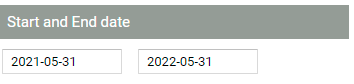
\includegraphics{./images/Figure1} 

}

\caption{Date Range TextBox}\label{fig:figG1}
\end{figure}

VICAL uses this interval to search for available Landsat or sentinel-2 images, and with these images estimate VIs. VICAL by default sets the end date as the current date and the start date one year ago to the current date.

\textbf{2) Cloud Percentage: } A maximum cloud threshold must be entered, by default it is set to 30\% (Figure \ref{fig:figG2}).

\begin{figure}

{\centering 
\includegraphics{./images/Figure2} 

}

\caption{Cloud Percentage Threshold}\label{fig:figG2}
\end{figure}

\textbf{3). Satellite: } four available options are derived from landsat and sentinel-2 satellites (described in the section \ref{Sat} \textbf{Satellites}) (Figure \ref{fig:figG3}):

\begin{figure}

{\centering 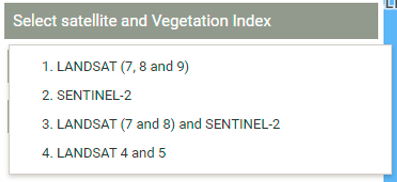
\includegraphics{./images/Figure3} 

}

\caption{Satellites and sensors available at VICAL}\label{fig:figG3}
\end{figure}

~\emph{\textbf{i) Landsat (7, 8 y 9):} returns Landsat images from sensors 7, 8 and 9 that are within the user-defined interval and with a maximum cloud threshold. Landsat 7 ETM+ data were spectrally fitted to Landsat 8 and 9 spectral bands (OLI and OLI-2) using the procedure recommended by \citep{Roy2016} to generate a single set of harmonized data.}

~\emph{\textbf{ii) Sentinel-2:} returns Sentinel-2 images that are within the user-defined interval and with the maximum cloud threshold.}

~\emph{\textbf{iii) Landsat (7, 8 y 9) and Sentinel-2}: Returns both Landsat (7, 8 and 9) and Sentinel-2 images. Sentinel-2 MSI data are spectrally fit to Landsat-8 and 9 (OLI and OLI-2) spectral bands using the procedure recommended by \citep{Claverie2018}. Landsat 7 ETM+ data were spectrally fitted to Landsat 8 and 9 spectral bands (OLI and OLI-2) using the procedure recommended by \citep{Roy2016}. In this way a single set of harmonized data is generated.}

~\emph{\textbf{iv) Landsat (4 y 5):} returns LandSat -4 and 5 images that are within the defined interval and with a maximum cloud threshold.}

\textbf{4). Vegetation index: } The user can select from 23 VIs commonly used in agricultural applications (Figure \ref{fig:figG4}), The formulas for each vegetation index are found in the section \ref{Iveg} \textbf{Vegetation Indices}.

\begin{figure}

{\centering 
\includegraphics{./images/Figure5} 

}

\caption{Vegetation Index Selector}\label{fig:figG4}
\end{figure}

\begin{figure}

{\centering 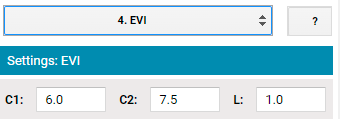
\includegraphics{./images/Figure5.1} 

}

\caption{Coeficientes de IV}\label{fig:figG5}
\end{figure}

\textbf{5) other additional functions: } VICAL allows you to select additional options (Figure \ref{fig:figG6}), for example:

\begin{figure}

{\centering 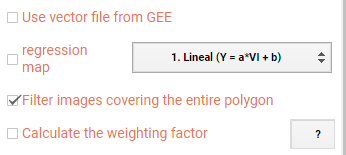
\includegraphics{./images/Figure9} 

}

\caption{Optional configuration in VICAL}\label{fig:figG6}
\end{figure}

\emph{\textbf{i) Use a GEE vector file:} As indicated in the initial part of this chapter, the user can use a GEE vector file (polygon type). For this option, you must enter a URL address (Table ID) of the vector file that has been uploaded to GEE (Figure \ref{fig:figG7}). in this way, even if there are digitized polygons, VICAL recognizes that the VIs must be calculated on the polygons of the vector file. }

\begin{figure}

{\centering 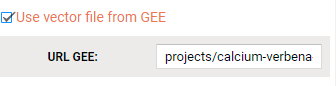
\includegraphics{./images/Figure10} 

}

\caption{Table ID of the GEE vector file}\label{fig:figG7}
\end{figure}

\emph{\textbf{ii) regression map:} The user obtains as a result a regression map based on the values of the calculated VIs. You can select between four types of functions: linear, quadratic, potential and exponential, and then you need to enter the adjustment coefficients for the selected function (Figure \ref{fig:figG8}).}

\begin{figure}

{\centering 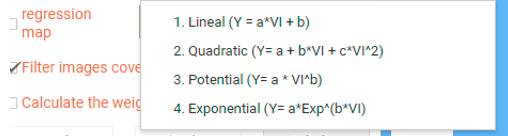
\includegraphics{./images/Figure8} 

}

\caption{Functions considered}\label{fig:figG8}
\end{figure}

\emph{\textbf{iii) Filter images that cover the entire polygon:} Images that completely cover the polygon(s) are filtered, otherwise images are displayed even if they cover a certain percentage of the polygon. This option is useful for polygons that cover large surfaces (hundreds of hectares).}\\
\emph{\textbf{iv) Calculate weighting factor (WF):} WF is the ratio of the VI value in a pixel to the average VI in the polygon (parcel). It is calculated for each digitized polygon. The WF in an agricultural parcel is a standardized indicator of the productive potential of each pixel of an image. }

\textbf{5) Calculate: }: When the options have been configured, click on \textbf{calculate} and at least three layers will be shown on the map: \emph{\textbf{i) RGB image of the first image found in the set interval, ii) VI map, iii) digitized polygons}. }

\hypertarget{using-digitized-polygons}{%
\section{Using digitized polygons}\label{using-digitized-polygons}}

The user can digitize any parcel (polygons) using the drawing tools found in the upper left corner of the map (Figure \ref{fig:figG9}). VICAL recognizes that VIs must be calculated on these polygons.

\begin{figure}

{\centering 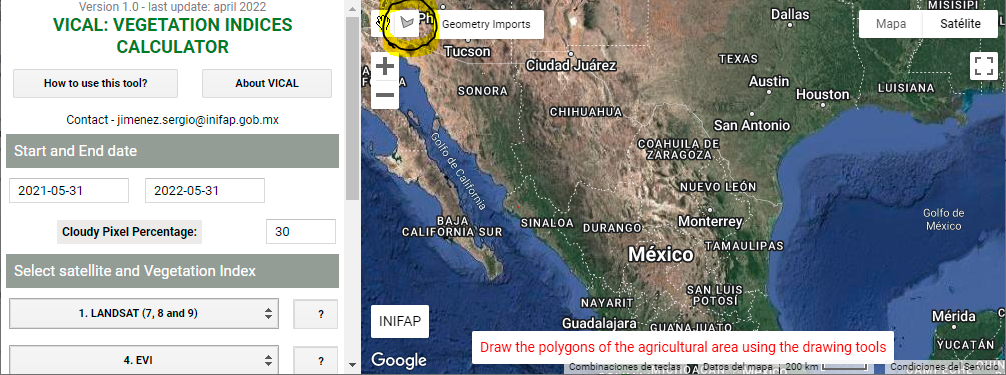
\includegraphics[width=0.75\linewidth]{./images/Figure11} 

}

\caption{Drawing tools}\label{fig:figG9}
\end{figure}

This option is useful when there are few parcels where you want to estimate VIs (Figure \ref{fig:figG10}). O bien, It is also useful when you want to download VIs for a particular area regardless of parcel boundaries. (Figure \ref{fig:figG11}).

To edit the polygon or create a new polygon, click on the \emph{``Edit and New Polygon''} buttons, respectively. These options are available after a calculation has been performed.

\begin{figure}

{\centering 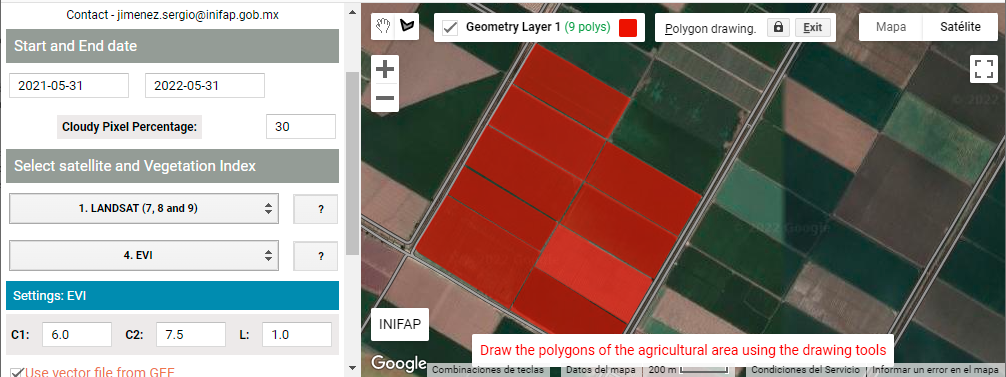
\includegraphics[width=0.75\linewidth]{./images/Figure12} 

}

\caption{Digitized parcels}\label{fig:figG10}
\end{figure}

\begin{figure}

{\centering 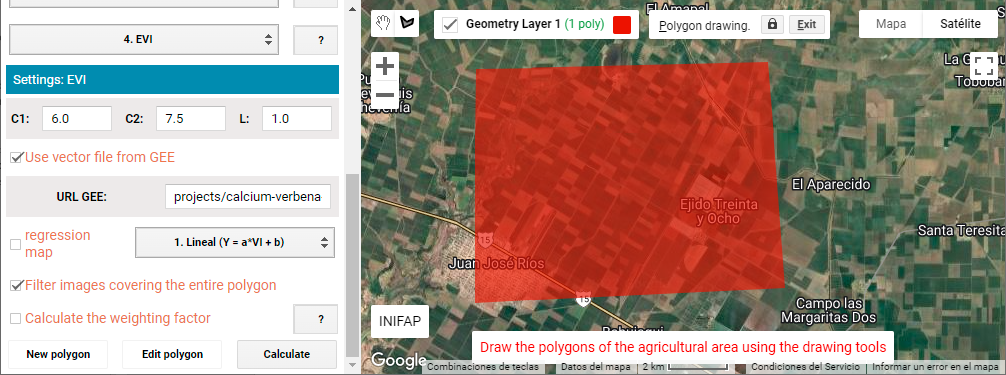
\includegraphics[width=0.75\linewidth]{./images/Figure13} 

}

\caption{poligono digitalizados}\label{fig:figG11}
\end{figure}

\hypertarget{using-gee-vector-file}{%
\section{Using GEE vector file}\label{using-gee-vector-file}}

For this option, the user must enter the \textbf{URL (Table ID)} of the vector file with which the calculations are to be performed; this indicates that you must have a GEE account and import a polygon-type vector file into your account.

The *Table ID\textbf{ can be obtained by left clicking on the file found in the }Assets** tab of your GEE account (Figure \ref{fig:figG12}).

\begin{figure}

{\centering 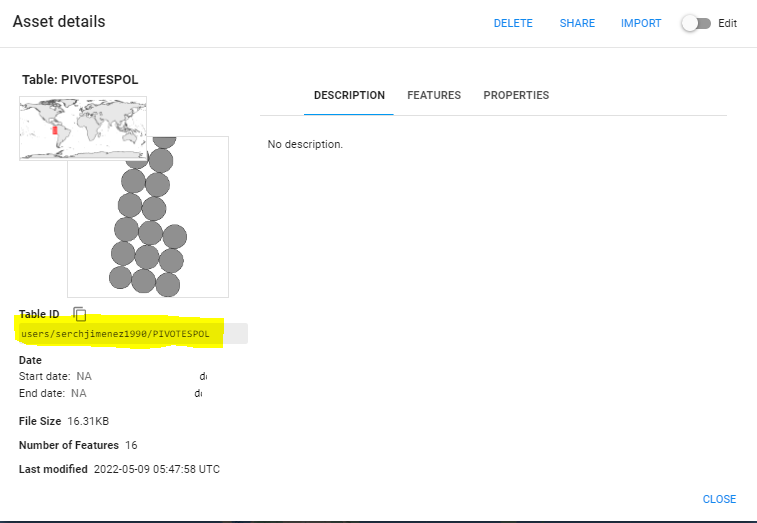
\includegraphics[width=0.75\linewidth]{./images/Figure14} 

}

\caption{vector file details}\label{fig:figG12}
\end{figure}

So that the vector file can be used in \textbf{VICAL}, you must have the ``Anyone can read'' box activated (Figure \ref{fig:figG13}).

\begin{figure}

{\centering 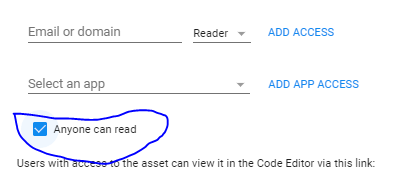
\includegraphics[width=0.75\linewidth]{./images/Figure6} 

}

\caption{Share option view}\label{fig:figG13}
\end{figure}

\hypertarget{implementation}{%
\chapter{implementation}\label{implementation}}

This section presents an example of how to navigate and how the VICAL results are displayed.

\hypertarget{PriVis}{%
\section{First views}\label{PriVis}}

When VIs are calculated using VICAL, a minimum of three mandatory and optional layers are shown on the map: (i) RGB combination \emph{(Figure \ref{fig:figI1})}, (ii)the selected VI \emph{(Figure \ref{fig:figI2})}, (iii) weighting factor (optional) calculated for each polygon \emph{(Figure \ref{fig:figI3})}, (iv) the regression map (optional) \emph{(Figure \ref{fig:figI4})} and (v) user drawn polygons. These maps, at first, are obtained from the first image found in the image collection..

The following images show some visualizations obtained from the URL that comes by default in VICAL ( \emph{``Use vector file from GEE''} was activated) and activating the linear regression option with coefficients of a=1.15 and b=0.17.

\begin{figure}

{\centering 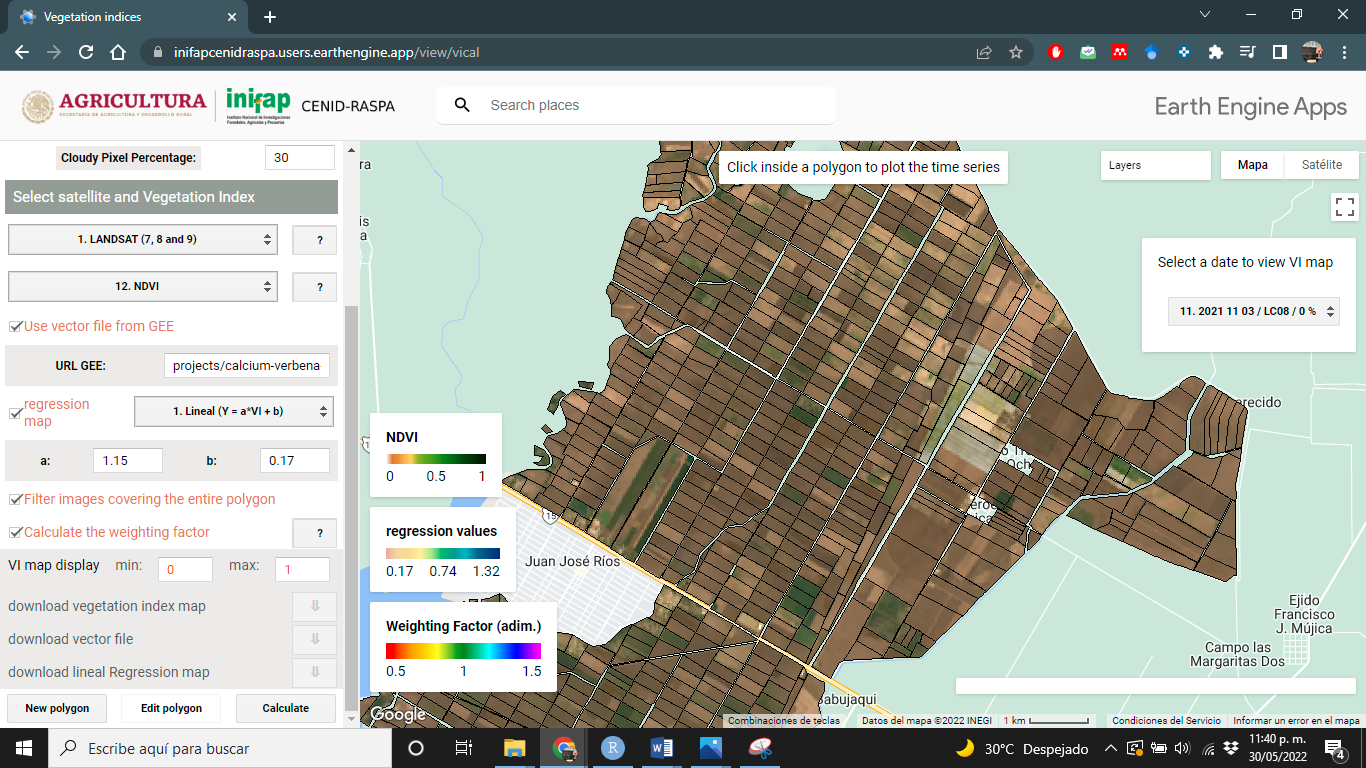
\includegraphics[width=0.85\linewidth]{./images/Figure51} 

}

\caption{RGB Combination}\label{fig:figI1}
\end{figure}

\begin{figure}

{\centering 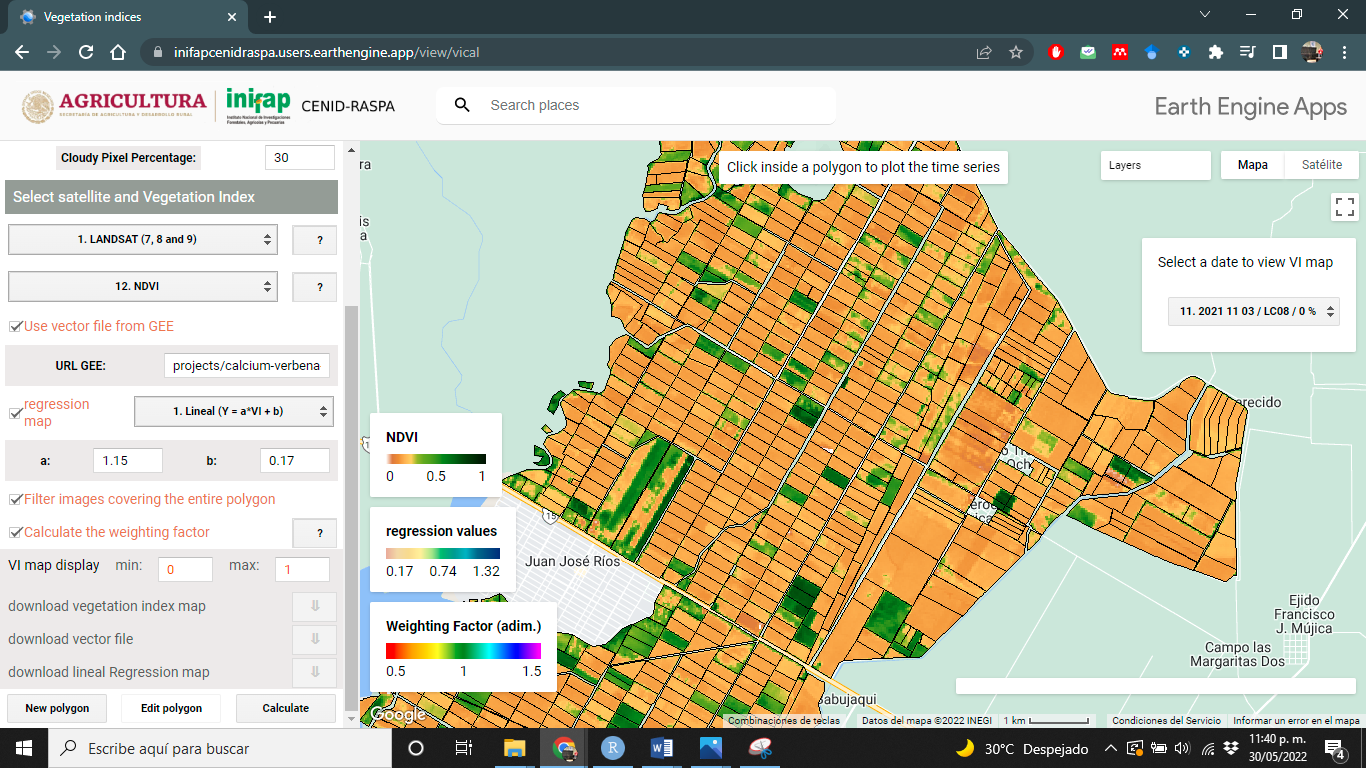
\includegraphics[width=0.85\linewidth]{./images/Figure52} 

}

\caption{NDVI map}\label{fig:figI2}
\end{figure}

\begin{figure}

{\centering 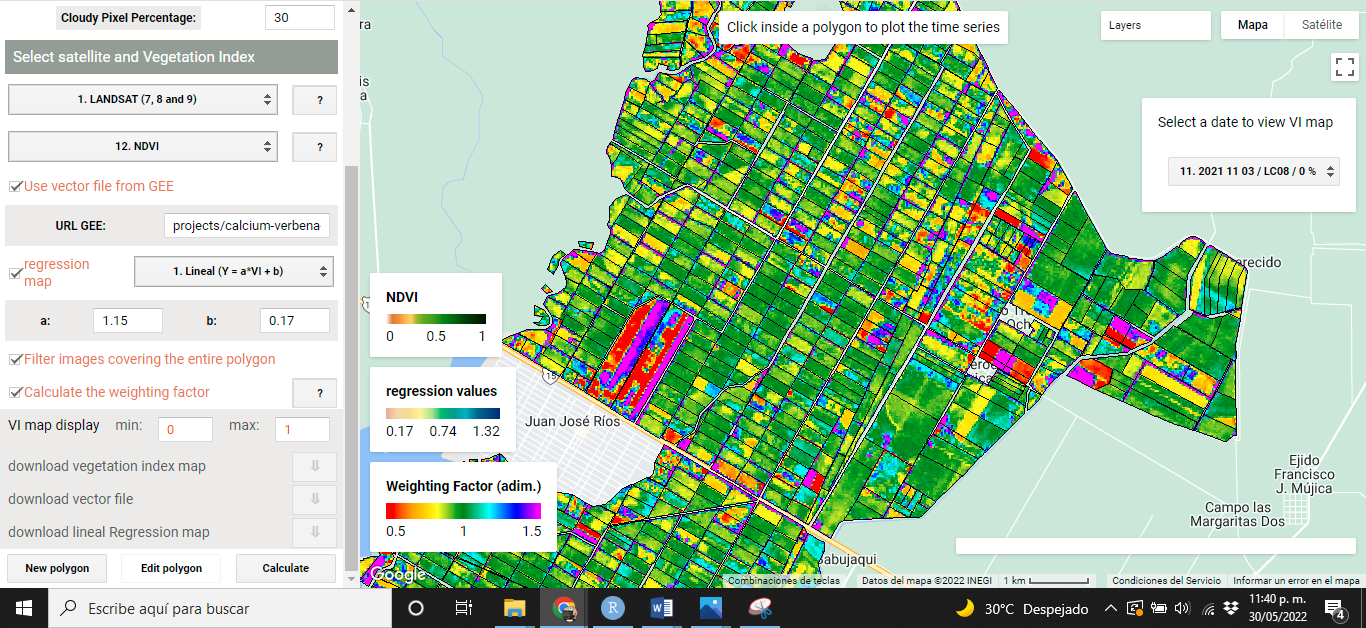
\includegraphics[width=0.85\linewidth]{./images/Figure53} 

}

\caption{Weighting factor (optional)}\label{fig:figI3}
\end{figure}

\begin{figure}

{\centering 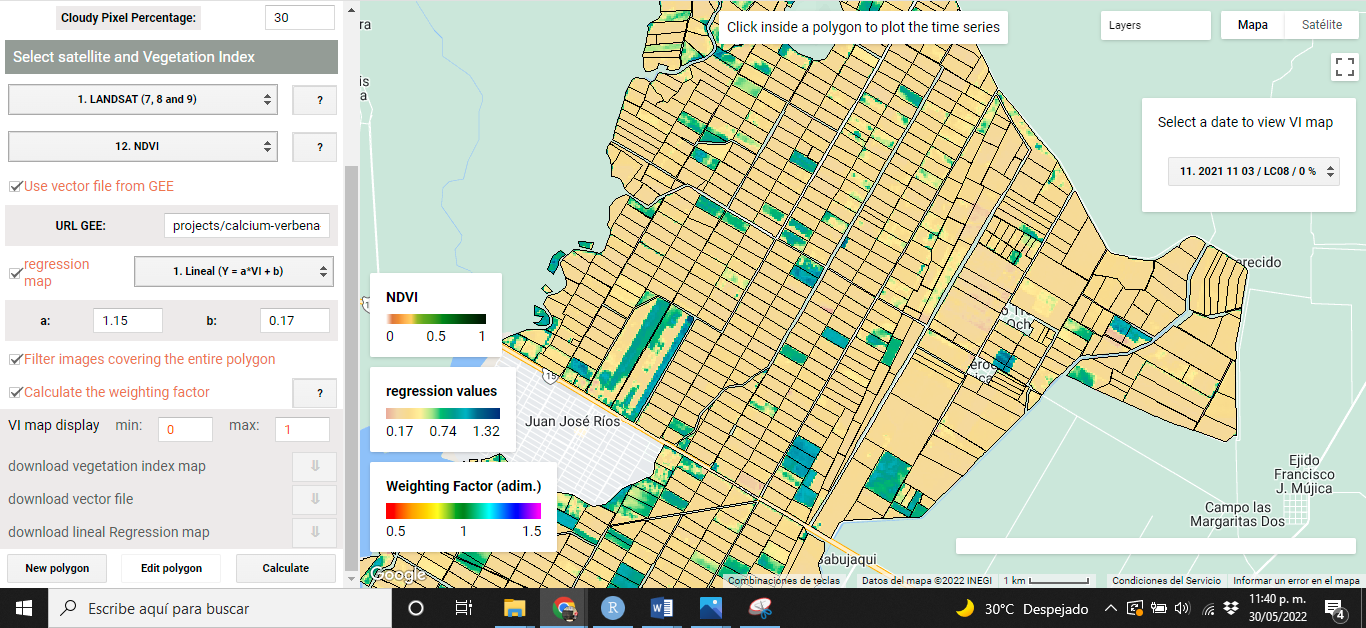
\includegraphics[width=0.85\linewidth]{./images/Figure54} 

}

\caption{Regression Map (optional)}\label{fig:figI4}
\end{figure}

\hypertarget{navigate-between-images}{%
\section{Navigate between images}\label{navigate-between-images}}

VICAL creates a images collection defined by the user's configuration; therefore, the user can navigate between the found images. To do this, a bar appears on the upper right side, where clicking on it displays a list where each row represents an image.

The short nomenclature used to name the images is: (Figure \ref{fig:figI5}): \emph{Image number found\textbf{+} point \textbf{+} Image date (starting with year, month and day)\textbf{+} / \textbf{+} Sensor \textbf{+} / \textbf{+} Cloud percentage in the image.}

\begin{figure}

{\centering 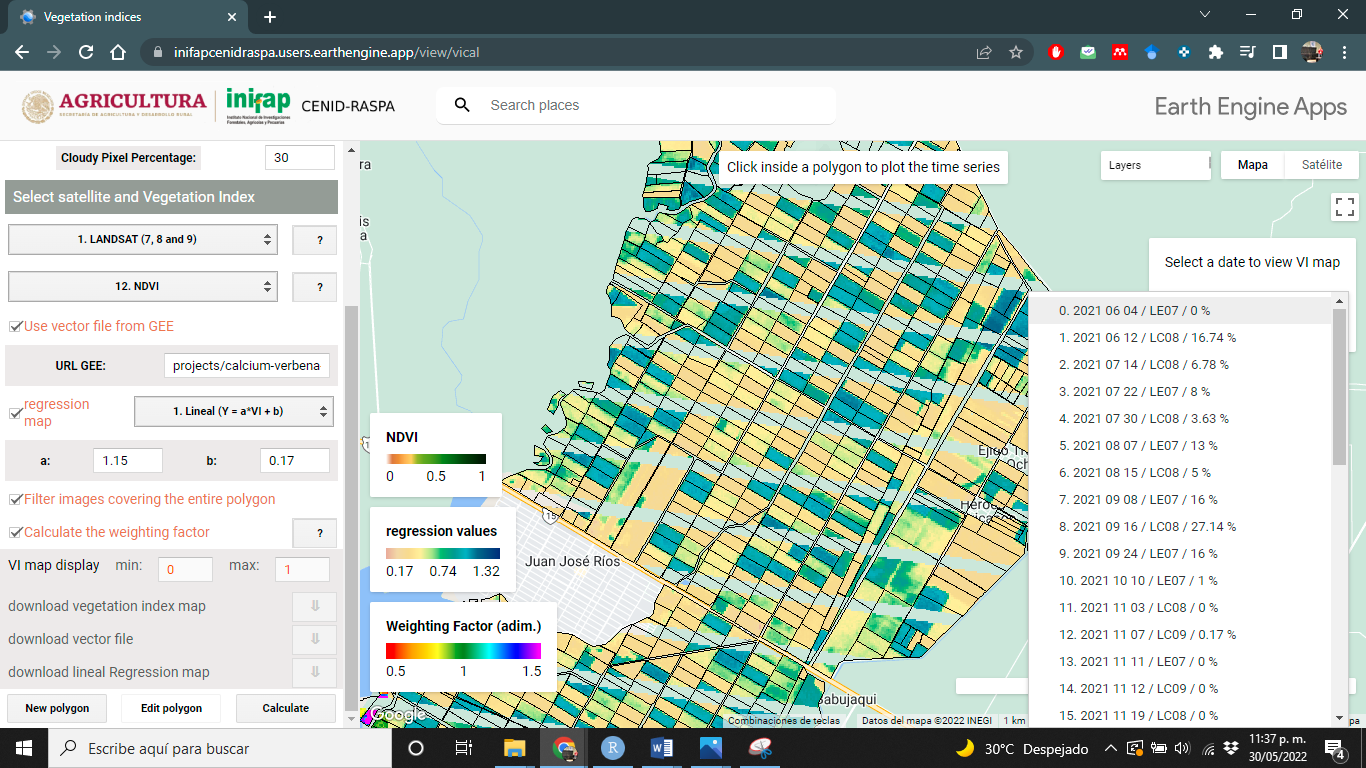
\includegraphics[width=0.85\linewidth]{./images/Figure55} 

}

\caption{List of images found}\label{fig:figI5}
\end{figure}

Click on any row you want to view and the layers described in section \ref{PriVis} will appear (Figure \ref{fig:figI6}).

\begin{figure}

{\centering 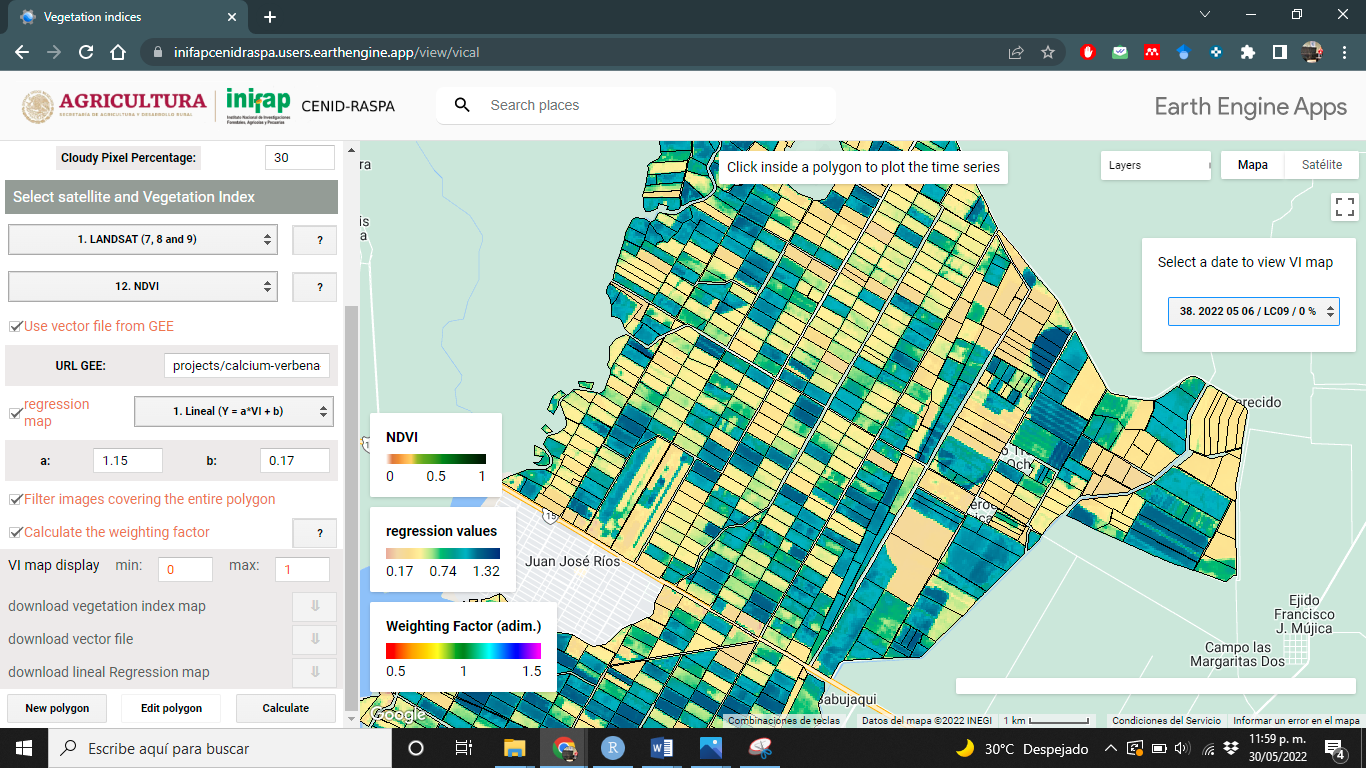
\includegraphics[width=0.85\linewidth]{./images/Figure56} 

}

\caption{Maps for the selected date}\label{fig:figI6}
\end{figure}

\hypertarget{vi-map-display}{%
\section{VI map display}\label{vi-map-display}}

The user can change the display values of the VI map by changing the range in which the \textbf{maximum} and \textbf{minimum} value varies, for this, it is necessary to enter the values in the option \emph{``VI map display''} (Figure \ref{fig:figI7}) and press the Enter key with the keyboard.

\begin{figure}

{\centering 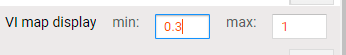
\includegraphics{./images/Figure57} 

}

\caption{IV map display setting}\label{fig:figI7}
\end{figure}

The program recognizes when the value is changed and automatically creates the layer with the new display values (Figure \ref{fig:figI8}). It is possible to change these display values after the user has navigated between images.

\begin{figure}

{\centering 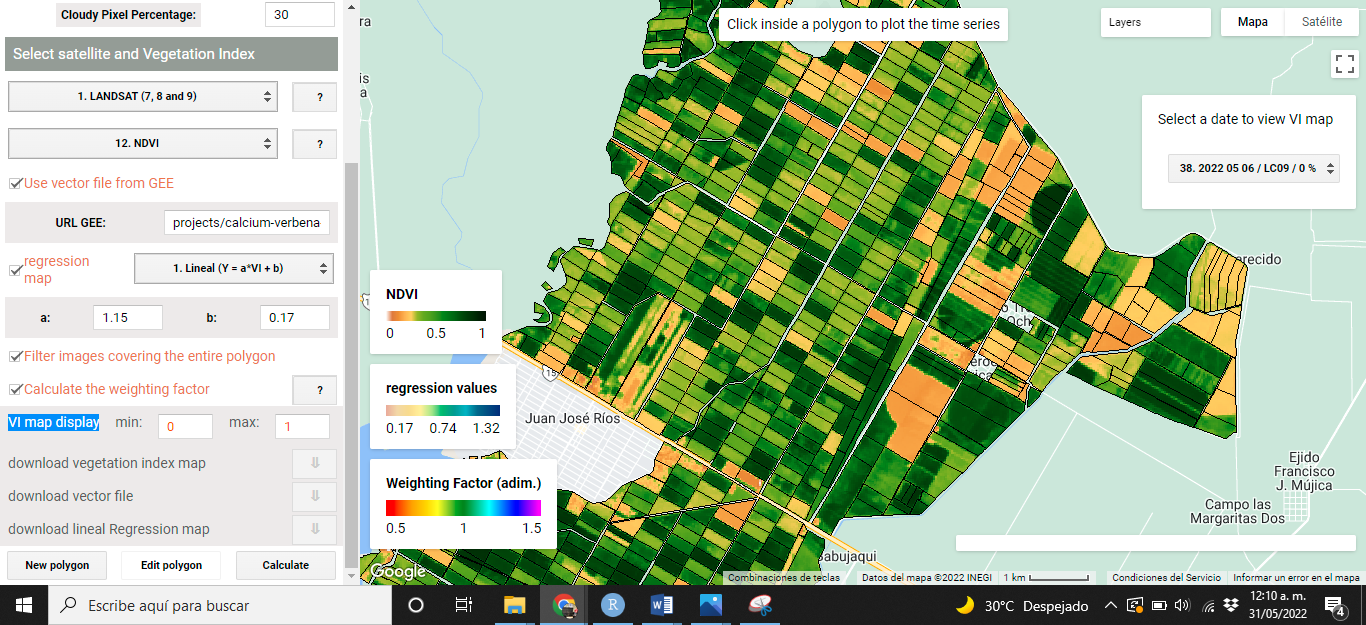
\includegraphics[width=0.85\linewidth]{./images/Figure58} 

}

\caption{NDVI with values in the range [0,1]}\label{fig:figI8}
\end{figure}

\begin{figure}

{\centering 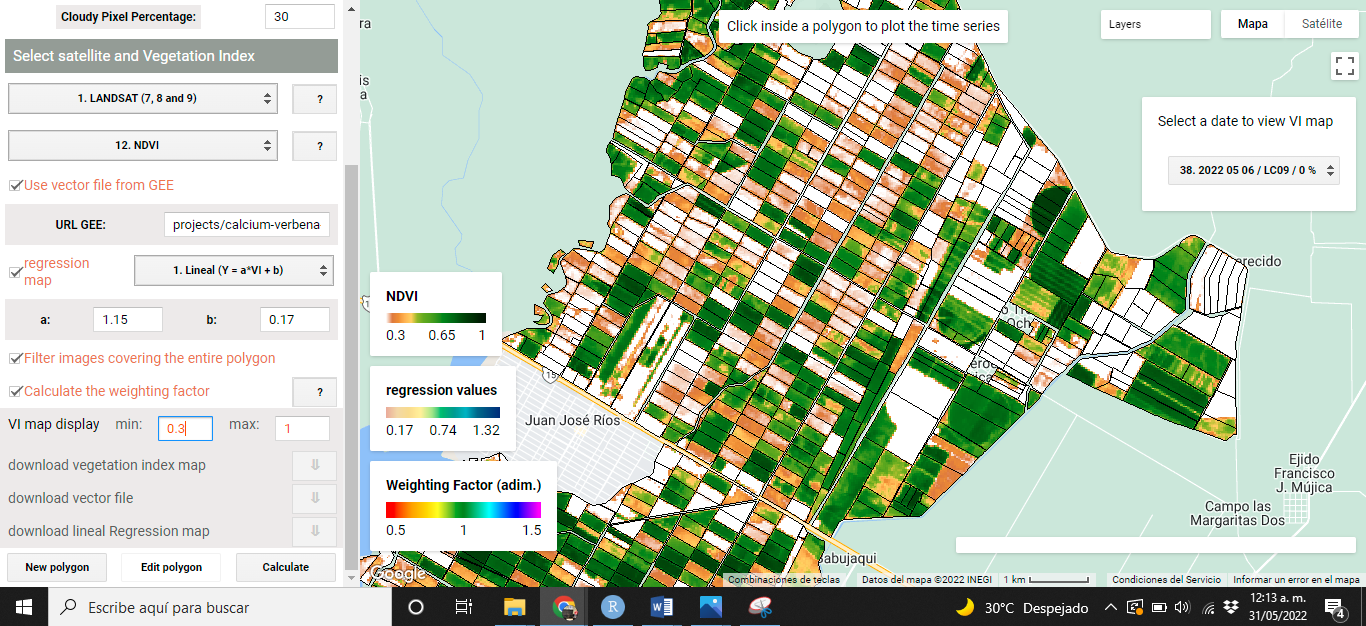
\includegraphics[width=0.85\linewidth]{./images/Figure59} 

}

\caption{NDVI with values in the range [0.3,1]}\label{fig:figI9}
\end{figure}

\hypertarget{time-series}{%
\section{Time series}\label{time-series}}

The VI time series is obtained by clicking inside any polygon, therefore, the values are only for the selected polygon. The time series is shown in a graph where the average and standard deviation of the IV values are calculated. each point of the graph represents an image found according to the user's configuration (Figure \ref{fig:figI10} y (Figure \ref{fig:figI11})).

\begin{figure}

{\centering 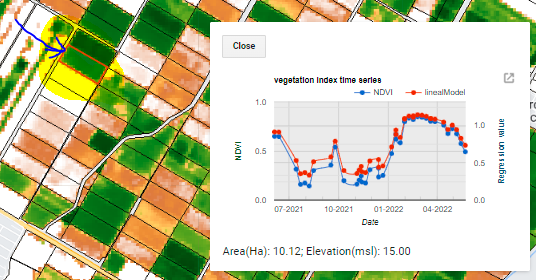
\includegraphics{./images/Figure60} 

}

\caption{IV time series for the plot indicated}\label{fig:figI10}
\end{figure}
\begin{figure}

{\centering 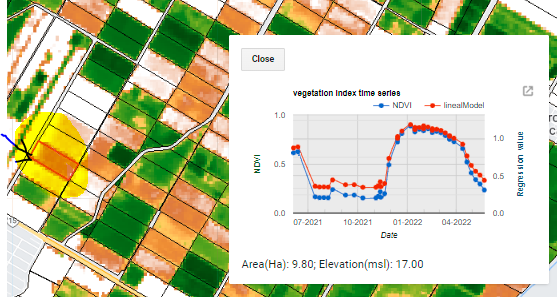
\includegraphics{./images/Figure61} 

}

\caption{IV time series for the plot indicated}\label{fig:figI11}
\end{figure}

\hypertarget{download-information}{%
\section{Download information}\label{download-information}}

Three layers of the five shown on the map can be downloaded. Download buttons are displayed at the bottom of the configuration section (Figure \ref{fig:figI12}). The layers that can be downloaded are:

\begin{figure}

{\centering 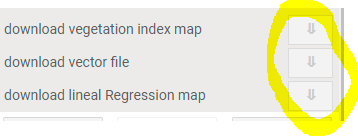
\includegraphics{./images/Figure62} 

}

\caption{download options}\label{fig:figI12}
\end{figure}

\textbf{i) VI map:} The Raster image is downloaded with VI values calculated and cropped for the area of interest. The download is done in TIF format, which can be viewed, for example, in QGIS \emph{(Figure \ref{fig:figI13})}.

\textbf{ii) vector file:} The digitized polygon is downloaded in kml format, which can be viewed, for example, in Google Earth.

\textbf{iii) regression map:} This option is available if ``regression map'' is activated; the raster image is downloaded with values of the regression map and cropped for the area of interest, the download is done in TIF format that can be viewed, for example, in QGIS.

\begin{figure}

{\centering 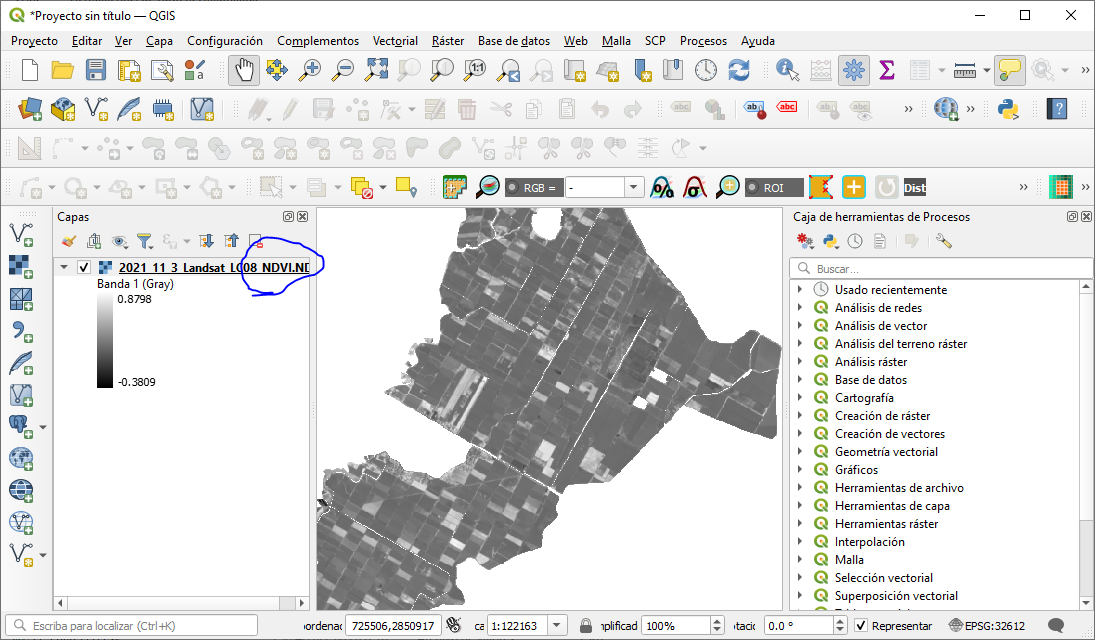
\includegraphics[width=0.85\linewidth]{./images/Figure63} 

}

\caption{NDVI image displayed in QGIS}\label{fig:figI13}
\end{figure}

\hypertarget{vical-in-gee}{%
\chapter{VICAL in GEE}\label{vical-in-gee}}

This section shows how to use the VICAL scripts to implement them in GEE.

VICAL has three main files that can be imported into a GEE Script, these are:

\begin{Shaded}
\begin{Highlighting}[]
\CommentTok{// Image collections}
\KeywordTok{var}\NormalTok{ imp }\OperatorTok{=} \PreprocessorTok{require}\NormalTok{(}\StringTok{\textquotesingle{}users/InifapCenidRaspa/VICAL:Exportaciones\textquotesingle{}}\NormalTok{)}\OperatorTok{;}
\CommentTok{// Vegetation indices}
\KeywordTok{var}\NormalTok{ imp2}\OperatorTok{=} \PreprocessorTok{require}\NormalTok{(}\StringTok{\textquotesingle{}users/InifapCenidRaspa/VICAL:VegetationIndex\textquotesingle{}}\NormalTok{)}\OperatorTok{;} 
\CommentTok{// visualization styles}
\KeywordTok{var}\NormalTok{ St}\OperatorTok{=} \PreprocessorTok{require}\NormalTok{(}\StringTok{\textquotesingle{}users/InifapCenidRaspa/VICAL:Style\textquotesingle{}}\NormalTok{)}\OperatorTok{;}
\end{Highlighting}
\end{Shaded}

\hypertarget{CImg}{%
\section{Image collection}\label{CImg}}

Before importing the image collections, some variables must be declared that are useful for filtering this collection: i) a point or polygon; ii) date range, and iii) cloud threshold value in images. These declarations are shown in the following code:

\begin{Shaded}
\begin{Highlighting}[]
\KeywordTok{var}\NormalTok{ fecha }\OperatorTok{=}\NormalTok{ [}\StringTok{\textquotesingle{}2021{-}01{-}01\textquotesingle{}}\OperatorTok{,} \StringTok{\textquotesingle{}2022{-}03{-}18\textquotesingle{}}\NormalTok{]}\OperatorTok{;} \CommentTok{//Start and end date }
\CommentTok{//polygon or point}
\KeywordTok{var}\NormalTok{ table }\OperatorTok{=}\NormalTok{ ee}\OperatorTok{.}\FunctionTok{FeatureCollection}\NormalTok{(}\StringTok{"projects/calcium{-}verbena{-}328905/assets/Bate"}\NormalTok{)}\OperatorTok{;}

\KeywordTok{var}\NormalTok{ p\_nubes}\OperatorTok{=} \DecValTok{30}\OperatorTok{;}\CommentTok{//percentage of clouds}
\end{Highlighting}
\end{Shaded}

\hypertarget{landsat}{%
\subsection{Landsat}\label{landsat}}

If you want to use cloud-free atmospherically corrected LandSat images (4, 5, 7, 8 and 9), you can use the following code. A function is created to join the image collections. To do this, use the \textbf{\emph{imp}} file.

\begin{Shaded}
\begin{Highlighting}[]
\KeywordTok{function} \FunctionTok{ColeccionImagenSR}\NormalTok{(fecha}\OperatorTok{,}\NormalTok{ recorte}\OperatorTok{,}\NormalTok{ umbral)}
\NormalTok{\{}
  \CommentTok{// image collections are imported using the "imp" file}
  \KeywordTok{var}\NormalTok{ L9sr }\OperatorTok{=}\NormalTok{ imp}\OperatorTok{.}\FunctionTok{ColeccionLandsatSR}\NormalTok{(fecha}\OperatorTok{,} \StringTok{\textquotesingle{}LC09\textquotesingle{}}\OperatorTok{,}\NormalTok{ recorte}\OperatorTok{,}\NormalTok{ umbral)}\OperatorTok{;}
  \KeywordTok{var}\NormalTok{ L8sr }\OperatorTok{=}\NormalTok{ imp}\OperatorTok{.}\FunctionTok{ColeccionLandsatSR}\NormalTok{(fecha}\OperatorTok{,} \StringTok{\textquotesingle{}LC08\textquotesingle{}}\OperatorTok{,}\NormalTok{ recorte}\OperatorTok{,}\NormalTok{ umbral)}\OperatorTok{;}
  \KeywordTok{var}\NormalTok{ L7sr }\OperatorTok{=}\NormalTok{ imp}\OperatorTok{.}\FunctionTok{ColeccionLandsatSR}\NormalTok{(fecha}\OperatorTok{,} \StringTok{\textquotesingle{}LE07\textquotesingle{}}\OperatorTok{,}\NormalTok{ recorte}\OperatorTok{,}\NormalTok{ umbral)}\OperatorTok{;}
  \KeywordTok{var}\NormalTok{ L5sr }\OperatorTok{=}\NormalTok{ imp}\OperatorTok{.}\FunctionTok{ColeccionLandsatSR}\NormalTok{(fecha}\OperatorTok{,} \StringTok{\textquotesingle{}LT05\textquotesingle{}}\OperatorTok{,}\NormalTok{ recorte}\OperatorTok{,}\NormalTok{ umbral)}\OperatorTok{;}
  \KeywordTok{var}\NormalTok{ L4sr }\OperatorTok{=}\NormalTok{ imp}\OperatorTok{.}\FunctionTok{ColeccionLandsatSR}\NormalTok{(fecha}\OperatorTok{,} \StringTok{\textquotesingle{}LT04\textquotesingle{}}\OperatorTok{,}\NormalTok{ recorte}\OperatorTok{,}\NormalTok{ umbral)}\OperatorTok{;}
  \CommentTok{//ETM and ETM+ data are spectral fit to OLI and OLI{-}2 }
  \KeywordTok{var}\NormalTok{ L7a }\OperatorTok{=}\NormalTok{ L7sr}\OperatorTok{.}\FunctionTok{map}\NormalTok{(imp}\OperatorTok{.}\AttributeTok{TMaOLI}\NormalTok{)}\OperatorTok{;}
  \KeywordTok{var}\NormalTok{ L5a }\OperatorTok{=}\NormalTok{ L5sr}\OperatorTok{.}\FunctionTok{map}\NormalTok{(imp}\OperatorTok{.}\AttributeTok{TMaOLI}\NormalTok{)}\OperatorTok{;}
  \KeywordTok{var}\NormalTok{ L4a }\OperatorTok{=}\NormalTok{ L4sr}\OperatorTok{.}\FunctionTok{map}\NormalTok{(imp}\OperatorTok{.}\AttributeTok{TMaOLI}\NormalTok{)}\OperatorTok{;}
  \CommentTok{// Join collections}
  \KeywordTok{var}\NormalTok{ serieT }\OperatorTok{=}\NormalTok{L9sr}\OperatorTok{.}\FunctionTok{merge}\NormalTok{(L8sr)}\OperatorTok{.}\FunctionTok{merge}\NormalTok{(L7a)}\OperatorTok{.}\FunctionTok{merge}\NormalTok{(L5a)}\OperatorTok{.}\FunctionTok{merge}\NormalTok{(L4a)}\OperatorTok{.}\FunctionTok{sort}\NormalTok{(}\StringTok{\textquotesingle{}system:time\_start\textquotesingle{}}\NormalTok{)}\OperatorTok{;}
    \ControlFlowTok{return}\NormalTok{ serieT}\OperatorTok{;}
\NormalTok{\}}
\CommentTok{//The collection is imported using the previous function }
\KeywordTok{var}\NormalTok{ l8Sergio}\OperatorTok{=}\FunctionTok{ColeccionImagenSR}\NormalTok{(fecha}\OperatorTok{,}\NormalTok{ table}\OperatorTok{,}\NormalTok{ p\_nubes)}\OperatorTok{;}
\CommentTok{//we can print the images using the print() function to see if the }
\CommentTok{//filtering of the image collection has been carried out (Figure 6.1) }
\FunctionTok{print}\NormalTok{ (l8Sergio)}\OperatorTok{;}
\end{Highlighting}
\end{Shaded}

With these image collections, time series of different vegetation indices can be calculated.

\begin{figure}

{\centering 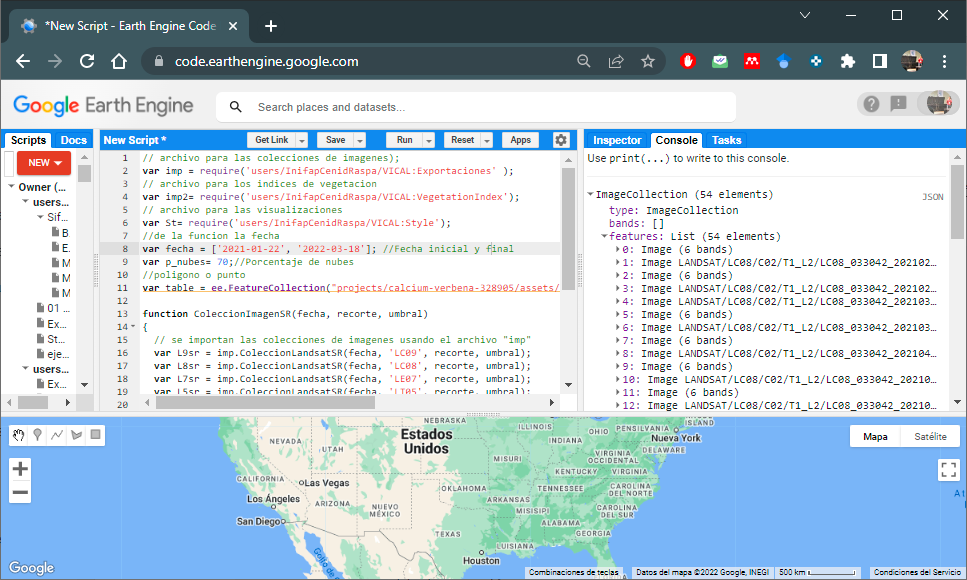
\includegraphics[width=0.85\linewidth]{./images/Figure70} 

}

\caption{Landsat Image Collection}\label{fig:figV1}
\end{figure}

\hypertarget{sentinel-2}{%
\subsection{Sentinel-2}\label{sentinel-2}}

If you want to use cloud-free, atmospherically corrected Sentinel-2 images, you can use the following code.

\begin{Shaded}
\begin{Highlighting}[]
\CommentTok{//The collection of images is imported using the following code}
\KeywordTok{var}\NormalTok{ S2sr }\OperatorTok{=}\NormalTok{ imp}\OperatorTok{.}\FunctionTok{ColeccionImagenSentinelSR}\NormalTok{(fecha}\OperatorTok{,}\NormalTok{ table}\OperatorTok{,}\NormalTok{ p\_nubes)}\OperatorTok{;}
\CommentTok{//we can print the images using the print() function to see if the }
\CommentTok{//filtering of the image collection has been carried out (Figure 6.2)}
\FunctionTok{print}\NormalTok{ (S2sr)}\OperatorTok{;}
\end{Highlighting}
\end{Shaded}

\begin{figure}

{\centering 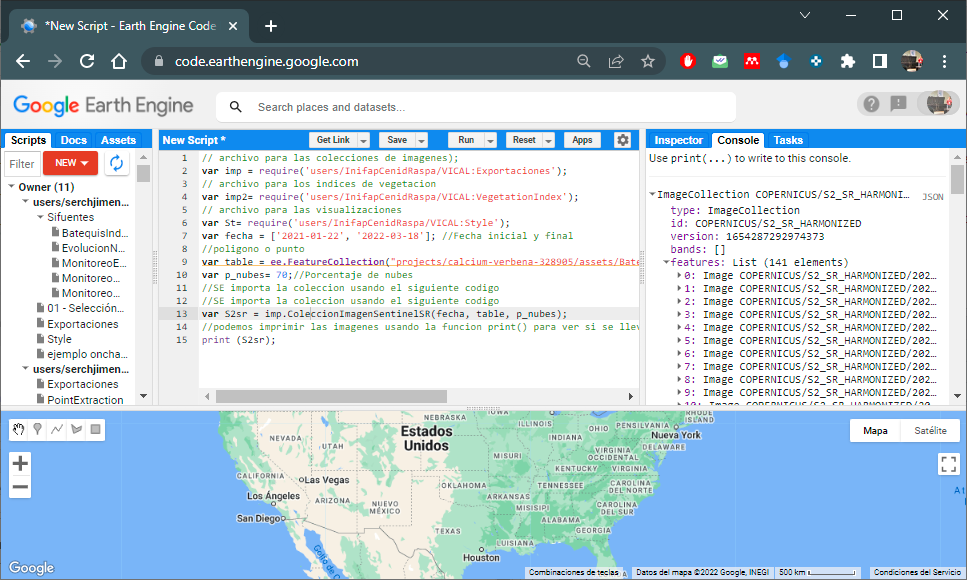
\includegraphics[width=0.85\linewidth]{./images/Figure71} 

}

\caption{Sentinel-2 Image Collection}\label{fig:figV2}
\end{figure}

\hypertarget{LanSen}{%
\subsection{Landsat y Sentinel-2}\label{LanSen}}

If you want to use cloud-free, atmospherically corrected LandSat and Sentinel-2 images, you can use the following code, data were spectrally fit to Landsat 8 bands. The functions described in Section \ref{CImg}:

\begin{Shaded}
\begin{Highlighting}[]
\KeywordTok{function} \FunctionTok{ColeccionImagenAMBOS}\NormalTok{(fecha}\OperatorTok{,}\NormalTok{ recorte}\OperatorTok{,}\NormalTok{ umbral)}
\NormalTok{\{}
  \CommentTok{//Function for Landsat images with spectral adjustment}
  \KeywordTok{var}\NormalTok{ L8Conjunto}\OperatorTok{=}\FunctionTok{ColeccionImagenSR}\NormalTok{(fecha}\OperatorTok{,}\NormalTok{ recorte}\OperatorTok{,}\NormalTok{ umbral)}
  \CommentTok{//Sentinel}
  \KeywordTok{var}\NormalTok{ S2sr }\OperatorTok{=}\NormalTok{ imp}\OperatorTok{.}\FunctionTok{ColeccionImagenSentinelSR}\NormalTok{(fecha}\OperatorTok{,}\NormalTok{ recorte}\OperatorTok{,}\NormalTok{ umbral)}\OperatorTok{;}
  \CommentTok{//Spectral matching of sentinel{-}2 to Landsat}
  \KeywordTok{var}\NormalTok{ S2a }\OperatorTok{=}\NormalTok{ S2sr}\OperatorTok{.}\FunctionTok{map}\NormalTok{(imp}\OperatorTok{.}\AttributeTok{MSIaOLI}\NormalTok{)}\OperatorTok{;} 
  \KeywordTok{var}\NormalTok{ serieT }\OperatorTok{=}\NormalTok{ S2a}\OperatorTok{.}\FunctionTok{merge}\NormalTok{(L8Conjunto)}\OperatorTok{.}\FunctionTok{sort}\NormalTok{(}\StringTok{\textquotesingle{}system:time\_start\textquotesingle{}}\NormalTok{)}\OperatorTok{;}
    \ControlFlowTok{return}\NormalTok{ serieT}\OperatorTok{;}
\NormalTok{\}}

\CommentTok{//The collection is imported}
\KeywordTok{var}\NormalTok{ S2B }\OperatorTok{=} \FunctionTok{ColeccionImagenAMBOS}\NormalTok{(fecha}\OperatorTok{,}\NormalTok{ table}\OperatorTok{,}\NormalTok{ p\_nubes)}\OperatorTok{;}
\CommentTok{//we can print the images using the print() function to see if the }
\CommentTok{//filtering of the image collection has been carried out (Figure 6.3)}
\FunctionTok{print}\NormalTok{ (S2sr)}\OperatorTok{;}
\end{Highlighting}
\end{Shaded}

\begin{figure}

{\centering 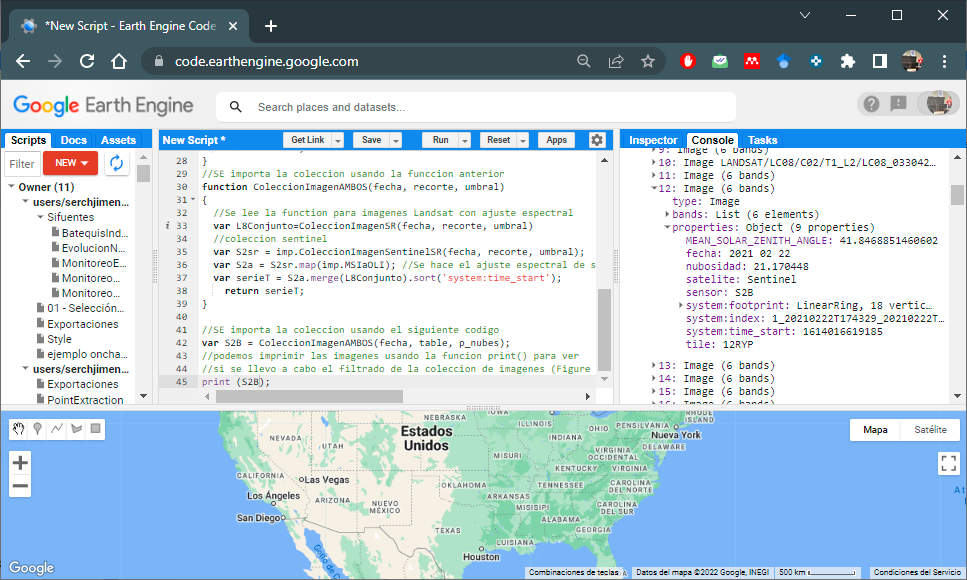
\includegraphics[width=0.85\linewidth]{./images/Figure72} 

}

\caption{Landsat and Sentinel-2 imagery collection}\label{fig:figV3}
\end{figure}

To view an example script click \href{https://code.earthengine.google.com/1eb76041c45bccf238c28ee9a4bad955}{here}

\hypertarget{vegetation-indices}{%
\section{Vegetation indices}\label{vegetation-indices}}

To calculate some of the VIs of \textbf{VICAL} you have to use the file \textbf{imp2}; and these VIs are imported using the names of the \textbf{ExpresionGEE} column that are shown in the \textbf{Table \ref{tab:Index}}.

For example, to calculate NDVI with LandSat and Sentinel-2 images from section \ref{LanSen}, the following code would be used:

\begin{Shaded}
\begin{Highlighting}[]
\CommentTok{//Normalized Difference Vegetation Index{-} NDVI}
\KeywordTok{var}\NormalTok{ ivs }\OperatorTok{=}\NormalTok{ ee}\OperatorTok{.}\FunctionTok{ImageCollection}\NormalTok{(S2B}\OperatorTok{.}\FunctionTok{map}\NormalTok{(imp2}\OperatorTok{.}\AttributeTok{NDVI}\NormalTok{))}\OperatorTok{;}
\CommentTok{//Print and view the NDVI band}
\FunctionTok{print}\NormalTok{ (ivs)}\OperatorTok{;}
\end{Highlighting}
\end{Shaded}

Figure \ref{fig:figV4} shows a single band called \textbf{NDVI}, calculated with the collection of images of the harmonized set

\begin{figure}

{\centering 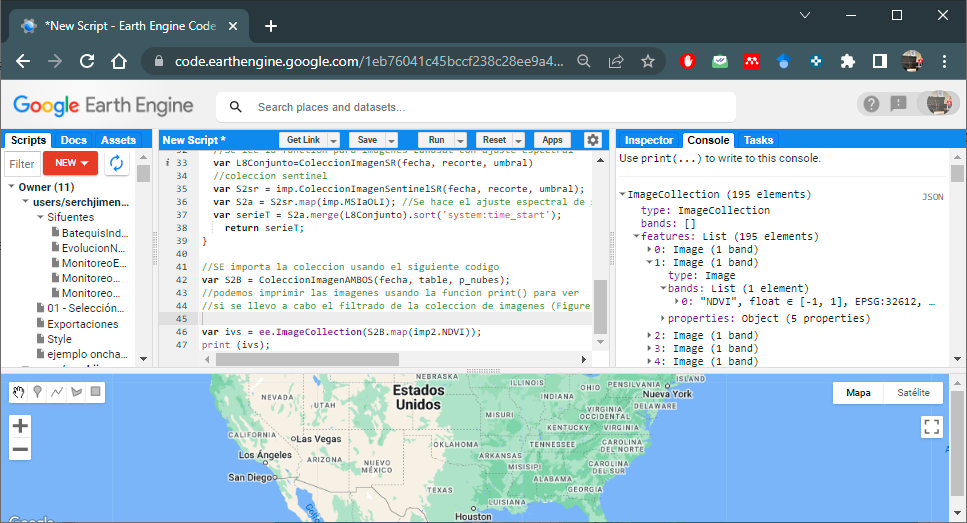
\includegraphics[width=0.85\linewidth]{./images/Figure73} 

}

\caption{NDVI Band Image Collection}\label{fig:figV4}
\end{figure}

The following code shows an example to display on the map the \textbf{NDVI} of the first image of the collection and cropped for the area. The \textbf{st} file of ¨\textbf{VICAL} is used.

\begin{Shaded}
\begin{Highlighting}[]
\CommentTok{//NDVI from the first image in the collection}
\KeywordTok{var}\NormalTok{ iv }\OperatorTok{=}\NormalTok{ ivs}\OperatorTok{.}\FunctionTok{first}\NormalTok{()}\OperatorTok{;}
\CommentTok{//Color palette where \textquotesingle{}st\textquotesingle{} file is used}
\KeywordTok{var}\NormalTok{ ivVis }\OperatorTok{=}\NormalTok{ \{}\DataTypeTok{min} \OperatorTok{:}\DecValTok{0}\OperatorTok{,} \DataTypeTok{max} \OperatorTok{:} \DecValTok{1}\OperatorTok{,} \DataTypeTok{palette} \OperatorTok{:}\NormalTok{ St}\OperatorTok{.}\AttributeTok{paletaIV}\NormalTok{\}}\OperatorTok{;}
\BuiltInTok{Map}\OperatorTok{.}\FunctionTok{addLayer}\NormalTok{(iv}\OperatorTok{.}\FunctionTok{clip}\NormalTok{(table)}\OperatorTok{,}\NormalTok{ ivVis}\OperatorTok{,}\StringTok{\textquotesingle{}NDVI\textquotesingle{}}\NormalTok{)}\OperatorTok{;} \CommentTok{//Indice}
\CommentTok{//the map is centered to the area}
 \BuiltInTok{Map}\OperatorTok{.}\FunctionTok{centerObject}\NormalTok{(table}\OperatorTok{,} \DecValTok{13}\NormalTok{)}\OperatorTok{;}
\end{Highlighting}
\end{Shaded}

Figure \ref{fig:figV6} shows the NDVI map for the area of interest

\begin{figure}

{\centering 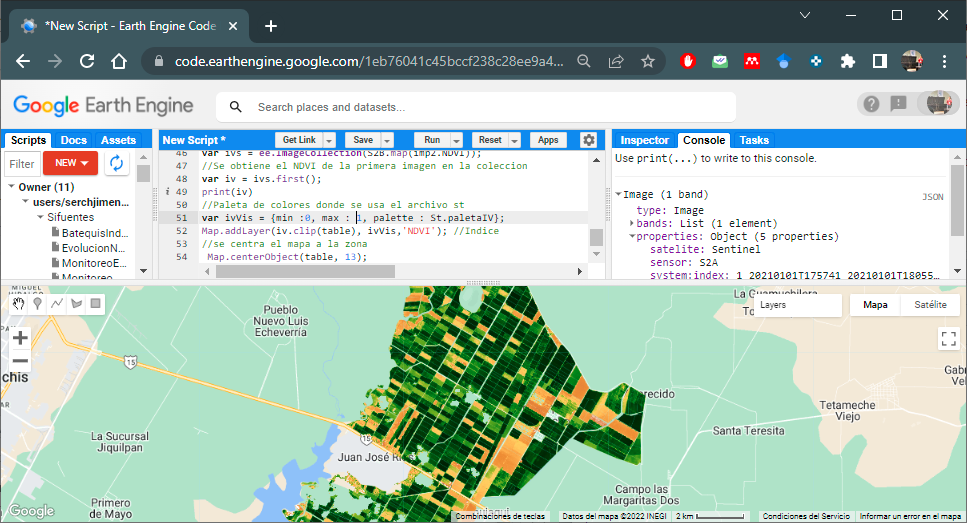
\includegraphics[width=0.85\linewidth]{./images/Figure74} 

}

\caption{NDVI map for the area of interest}\label{fig:figV6}
\end{figure}

To view the sample code click \href{https://code.earthengine.google.com/299b022150c4569d006b323931f8d828}{here}

If you want to display the NDVI of a particular image, you must convert it to a list.

\begin{table}

\caption{\label{tab:Index}Code of vegetation indices considered in VICAL}
\centering
\begin{tabular}[t]{lcccc}
\toprule
Number & Index & Abbreviation & ExpresionGEE & Coefficients\\
\midrule
1 & Atmospherically resistant vegetation index & ARVI* & ARVI & γ=1.0\\
2 & Adjusted transformed soil-adjusted vegetation index & ATSAVI* & ATSAVI & \\
3 & Difference vegetation index & DVI & DVI & \\
4 & Enhanced vegetation index & EVI & EVI & C1=6.0, C2= 7.5; L=1.0\\
5 & Enhanced vegetation index & EVI2* & EVI2 & C1=2.4\\
\addlinespace
6 & Green normalized difference vegetation index & GNDVI & GNDVI & \\
7 & Modified soil adjusted vegetation index & MSAVI2 & MSAVI2 & \\
8 & Moisture stress index & MSI & MSI & \\
9 & Modified triangular vegetation index & MTVI & MTVI & \\
10 & Modified triangular vegetation index-2 & MTVI2 & MTVI2 & \\
\addlinespace
 &  &  &  & \\
11 & Normalized difference tillage index (NDTI) & NDTI & NDTI & \\
12 & Normalized difference vegetation index & NDVI & NDVI & \\
13 & Normalized difference water index & NDWI & NDWI & \\
14 & Optimized soil adjusted vegetation index & OSAVI* & OSAVI & X=0.16\\
\addlinespace
15 & Renormalized difference vegetation index & RDVI & RDVI & \\
16 & Redness index & RI & RI & \\
17 & Ratio vegetation index & RVI & RVI & \\
18 & Soil adjusted vegetation index & SAVI* & SAVI & L=0.5\\
19 & Triangular vegetation index & TVI & TVI & \\
\addlinespace
20 & Transformed soil adjusted vegetation index & TSAVI* & TSAVI & a= 1 ; b=0;\\
21 & Visible atmospherically resistant index & VARI & VARI & \\
22 & Vegetation index number or simple ratio & VIN & VIN & \\
23 & Wide dynamic range vegetation index & WDRVI* & WDRVI & α=0.2\\
\bottomrule
\end{tabular}
\end{table}

\hypertarget{github-repository}{%
\section{GithUb repository}\label{github-repository}}

VICAL codes are written in JavaScript and are freely available on GitHub (\url{https://www.github.com/CenidRaspaRiego/VICAL} (accessed on 16 June 2022))

\hypertarget{citation}{%
\chapter{Citation}\label{citation}}

\href{https://www.mdpi.com/2073-4395/12/7/1518}{Jiménez-Jiménez, S.I.; Marcial-Pablo, M.d.J.; Ojeda-Bustamante, W.; Sifuentes-Ibarra, E.; Inzunza-Ibarra, M.A.; Sánchez-Cohen, I. VICAL: Global Calculator to Estimate Vegetation Indices for Agricultural Areas with Landsat and Sentinel-2 Data. Agronomy 2022, 12, 1518. https://doi.org/10.3390/agronomy12071518}

\hypertarget{updates}{%
\chapter{Updates}\label{updates}}

f you have questions or find that updates introduce errors, please post an issue in the VICAL GitHub repository - if you don't have a GitHub account, email Sergio at: \href{mailto:jimenez.sergio@inifap.gob.mx}{\nolinkurl{jimenez.sergio@inifap.gob.mx}}.

\hypertarget{may-02-2022}{%
\section{May 02, 2022}\label{may-02-2022}}

-The user can enter the \textbf{URL} (ID) of a vector file uploaded from GEE.
-The digitized polygon can be exported in \emph{.kml.} format

  \bibliography{book.bib,packages.bib}

\end{document}
